\usepackage{etex} %эта магическая херь избавляет от переполнения регистров TeX а!!!

\mode<article>{\usepackage{fullpage}}
\mode<presentation>{
    \usetheme{Madrid}
    \useoutertheme{shadow}
} 

\usepackage[utf8]{inputenc}
\usepackage[russian]{babel}
\usepackage{indentfirst}
\usepackage{graphicx}

\usepackage{amsmath}
\usepackage{amsfonts}
\usepackage{amsthm}
%\usepackage{algorithm}
%\usepackage{algorithmic}

%\usepackage[all]{xy}

\date{Лекция по дисциплине <<методы и средства защиты компьютерной информации>> (\today)}
\author[М.~М.~Шихов]{Михаил Шихов \\ \texttt{\underline{m.m.shihov@gmail.com}}}

%%для рисования графов пакетом xy-pic
%\entrymodifiers={++[o][F-]}

%%для псевдокода алгоритмов (algorithm,algorithmic)
%\renewcommand{\algorithmicrequire}{\textbf{Вход:}}
%\renewcommand{\algorithmicensure}{\textbf{Выход:}}
%\renewcommand{\algorithmiccomment}[1]{// #1}
%\floatname{algorithm}{Псевдокод}

%\setbeamercolor{alerted text}{fg=-green} %gyan, blue, green, -green

\usepackage[all]{xy}
\entrymodifiers={++[o][F-]}


\title[Безопасность в сети]{Безопасность в сети}


\begin{document}

\mode<article>{\maketitle\tableofcontents}
\frame<presentation>{\titlepage}
\begin{frame}<presentation>[allowframebreaks]
    \frametitle{Содержание}
    \tableofcontents
\end{frame}


\section{Теоретические основы}

\subsection{Пакетная передача данных и стеки протоколов}

\begin{frame}
    \frametitle{Коммутация пакетов vs коммутация сообщений}

    \begin{tabular}{cc}
        \raisebox{3\height}{
            {\xymatrix@=10pt{
                A \ar[dr] \ar@{.>}@/_10pt/[rrr]^{M_{AB}}
                    & *{} 
                        & *{} 
                            & B 
                                \\
                *{} 
                    & T_1 \ar[r]
                        & T_2 \ar[ur] \ar[dr]
                            & *{} 
                                \\
                C \ar[ur] \ar@{.>}@/^10pt/[rrr]_{M_{CD}}
                    & *{} 
                        & *{} 
                            & D 
            }}
        }
            &
                \begin{tabular}{c}
                    Коммутация сообщений\\
                    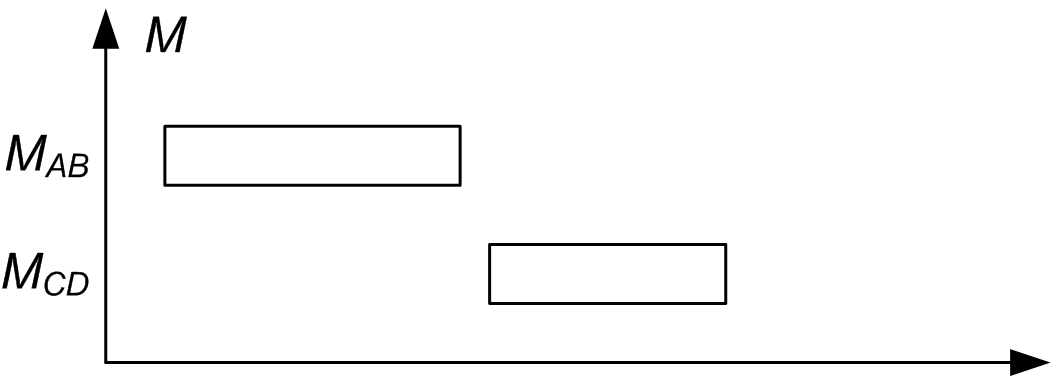
\includegraphics[width=0.5\textwidth]{fig/message}\\
                    \\
                    Коммутация пакетов\\
                    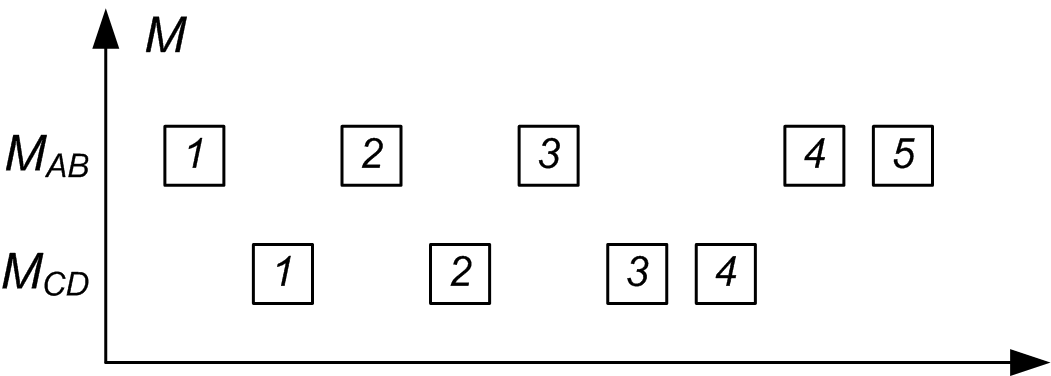
\includegraphics[width=0.5\textwidth]{fig/packet}
                \end{tabular}
    \end{tabular}
\end{frame}


\begin{frame}
    \frametitle{Стек протоколов}
        
    \begin{table}
        \centering
        \begin{tabular}{|c|c|}
            \hline\hline
            ISO/OSI                         & TCP/IP\\ \hline\hline
            Прикладной(Application)         & Прикладной(Application)   \\ \cline{1-1}
            Представительный (Presentation) &                           \\ \cline{1-1}
            Сеансовый (Session)             &                           \\ \hline
            Транспортный (Transport)        & Транспортный (Transport)  \\ \hline
            Сетевой (Network)               & Сетевой (Network)         \\ \hline
            Канальный (Link)                & Канальный (Link)          \\ \hline
            Физический (Physical)           & Физический (Physical)     \\ \hline
        \end{tabular}
    \end{table}
\end{frame}


\begin{frame}
    \frametitle{Передача сообщения}
    
    \begin{table}
        \centering
        \begin{tabular}{clc}
            \hline\hline
            Передатчик & Уровень стека TCP/IP & Приёмник \\
            \hline\hline
            \uncover<1,10>{\alert{$M$}}
                & 5. \alert<1,9>{Прикладной(Application)}
                    &\uncover<9,10>{\alert{$M$}}\\
            \uncover<2>{\alert{$h_4$}$M_i$\alert{$t_4$}}
                & 4. \alert<2,8>{Транспортный (Transport)}
                    &\uncover<8>{\alert{$h_4$}$M_i$\alert{$t_4$}}\\
            \uncover<3>{\alert{$h_3$}$h_4M_it_4$\alert{$t_3$}}
                & 3. \alert<3,7>{Сетевой (Network)}
                    &\uncover<7>{\alert{$h_3$}$h_4M_it_4$\alert{$t_3$}}\\
            \uncover<4>{\alert{$h_2$}$h_3h_4M_it_4t_3$\alert{$t_2$}}
                & 2. \alert<4,6>{Канальный (Link)}
                    &\uncover<6>{\alert{$h_2$}$h_3h_4M_it_4t_3$\alert{$t_2$}}\\
            \uncover<5>{\alert{$\downarrow$}}
                & 1. \alert<5>{Физический (Physical)}
                    &\uncover<5>{\alert{$\uparrow$}}\\ \hline
        \end{tabular}
    \end{table}
    \uncover<10>{
        Транспортный уровень разбивает сообщение $M$ на \alert{пакеты} $\{M_i\}$. Пакет транспорта, не гарантирующего доставку, называется \alert{дейтаграммой} (datagram) --- так же называют и пакет сетвевого уровня. На канальном уровне пакет называют \alert{кадром}. Если пакет сетевого уровня не помещается в кадр канального, то он <<фрагментируется>> (разбивается на подпакеты) и тогда говорят о \alert{фрагменте}.
    }
\end{frame}


\subsection{Протоколы на разных уровнях стека}

\begin{frame}
    \frametitle{Протоколы на разных уровнях TCP/IP}
        
    \begin{table}
        \centering
        \begin{tabular}{|l|l|}
            \hline\hline
            Уровень TCP/IP              & Протоколы уровня\\
            \hline\hline
            Прикладной(Application)     & HTTP, FTP, SNMP, SSH, (D)DNS,\ldots \\ \hline
            Транспортный (Transport)    & TCP, UDP,\ldots \\ \hline
            Сетевой (Network)           & IPv4, IPv6, ICMP, ARP, OSPF,\ldots \\ \hline
            Канальный (Link)            & Ethernet, SLIP, Token Ring, ATM,\ldots \\ \hline
            Физический (Physical)       & Физ. среда и принципы кодирования\\ \hline
        \end{tabular}
    \end{table}
\end{frame}


\begin{frame}
    \frametitle{Мультиплексирование на уровнях стека TCP/IP}
    \[
        {\xymatrix@=10pt{
        *{\text{Пр.}}
            &POP3 
                & SMTP 
                    & HTTP 
                        & DNS 
                            & SNMP 
                                & DHCP 
                                    \\
        *{}
            &*{}
                &*{}
                    &*{}
                        &*{}
                            &*{}
                                &*{}
                                    \\                                    
        *{\text{Тр.}}
            &*{} 
                & TCP \ar[uul]^{110}\ar[uu]^{25}\ar[uur]^{80}\ar[uurr]_{53}
                    & *{} 
                        & *{}
                            & UDP \ar[uul]^{53}\ar[uu]^{161}_{162}\ar[uur]_{67,68}
                                & *{} 
                                    \\
        *{\text{Сет.}}
            &OSPF
                &*{}
                    &*{}
                        &ICMP
                            &*{}
                                &*{}
                                    \\
        *{}
            &*{}
                &*{}
                    &IP\ar[ull]^{89}\ar[uul]^{6}\ar[ur]^{1}\ar@/_18pt/[uurr]_(.8){17}
                        &*{}
                            &ARP
                                &*{}
                                    \\
        *{\text{Кан.}}
            &*{}
                &*{}
                    &*{}
                        &Ethernet\ar[ur]_{0x0806}\ar[ul]^{0x0800}_{0x86DD}
                            &*{}
                                &*{}
                                    \\
        *{\text{Физ.}}
            &*{}
                &*{}
                    &*{}
                        &\sim\ar[u]
                            &*{}
                                &*{}
                                    \\
        }}
    \]        
\end{frame}


\subsection{Устройства на разных уровнях стека}

\begin{frame}
    \frametitle{Некоторые устройства на разных уровнях стека}
        
    \begin{table}
        \centering
        \begin{tabular}{|l|l|}
            \hline\hline
            Уровень TCP/IP              & Устройства\\
            \hline\hline
            Прикладной
                & 
                \parbox{0.6\textwidth}{
                    \begin{itemize}
                        \item сервер (server), клиентский компьютер, принтер и т.д. 
                    \end{itemize}
                }
                    \\ \hline            
            Транспортный   & \\ \hline            
            Сетевой
                & 
                \parbox{0.5\textwidth}{
                    \begin{itemize}
                        \item маршрутизатор (router);
                        \item шлюз (gateway).
                    \end{itemize}
                }
                    \\ \hline
            Канальный
                &
                \parbox{0.7\textwidth}{
                    \begin{itemize}
                        \item коммутатор (switch), мост (bridge);
                        \item сетевая карта (NIC (Network Interface Card)).
                    \end{itemize}
                }
                    \\ \hline            
            Физический 
                &
                \parbox{0.6\textwidth}{
                    \begin{itemize}
                        \item повторитель (repeater).
                    \end{itemize}
                }
            \\ \hline
        \end{tabular}
    \end{table}
\end{frame}

\begin{frame}
    \frametitle{Адресация на разных уровнях стека TCP/IP}
        
    \begin{table}
        \centering
        \begin{tabular}{|l|l|}
            \hline\hline
            Уровень TCP/IP              & Адресация\\
            \hline\hline
            Прикладной
                & 
                \parbox{0.6\textwidth}{
                    \begin{itemize}
                        \item DNS. Domain Name System. \alert{mail.ru}.
                        \item NBNS. NetBIOS Name Service\footnote{WINS в Windows}. \alert{server}.
                    \end{itemize}
                }
                    \\ \hline            
            Транспортный   & \\ \hline            
            Сетевой
                & 
                \parbox{0.72\textwidth}{
                    \begin{itemize}
                        \item IPv4. \alert{192.168.100.101/24}.
                        \item IPv6. \alert{2001:0db8:11a3:09d7:1f34:8a2e:07a0:765d}
                    \end{itemize}
                }
                    \\ \hline
            Канальный
                &
                \parbox{0.7\textwidth}{
                    Адреса канального уровня.
                    \begin{itemize}
                        \item Ethernet MAC\footnote{Media Access Control}. \alert{00-24-54-AA-84-AA}
                    \end{itemize}
                }
                    \\ \hline            
            Физический & \\ \hline
        \end{tabular}
    \end{table}
\end{frame}

\begin{frame}
    \frametitle{Локальная сеть. Обмен в пределах канала}
    \framesubtitle{Адресация канального уровня}
    
    \begin{figure}
        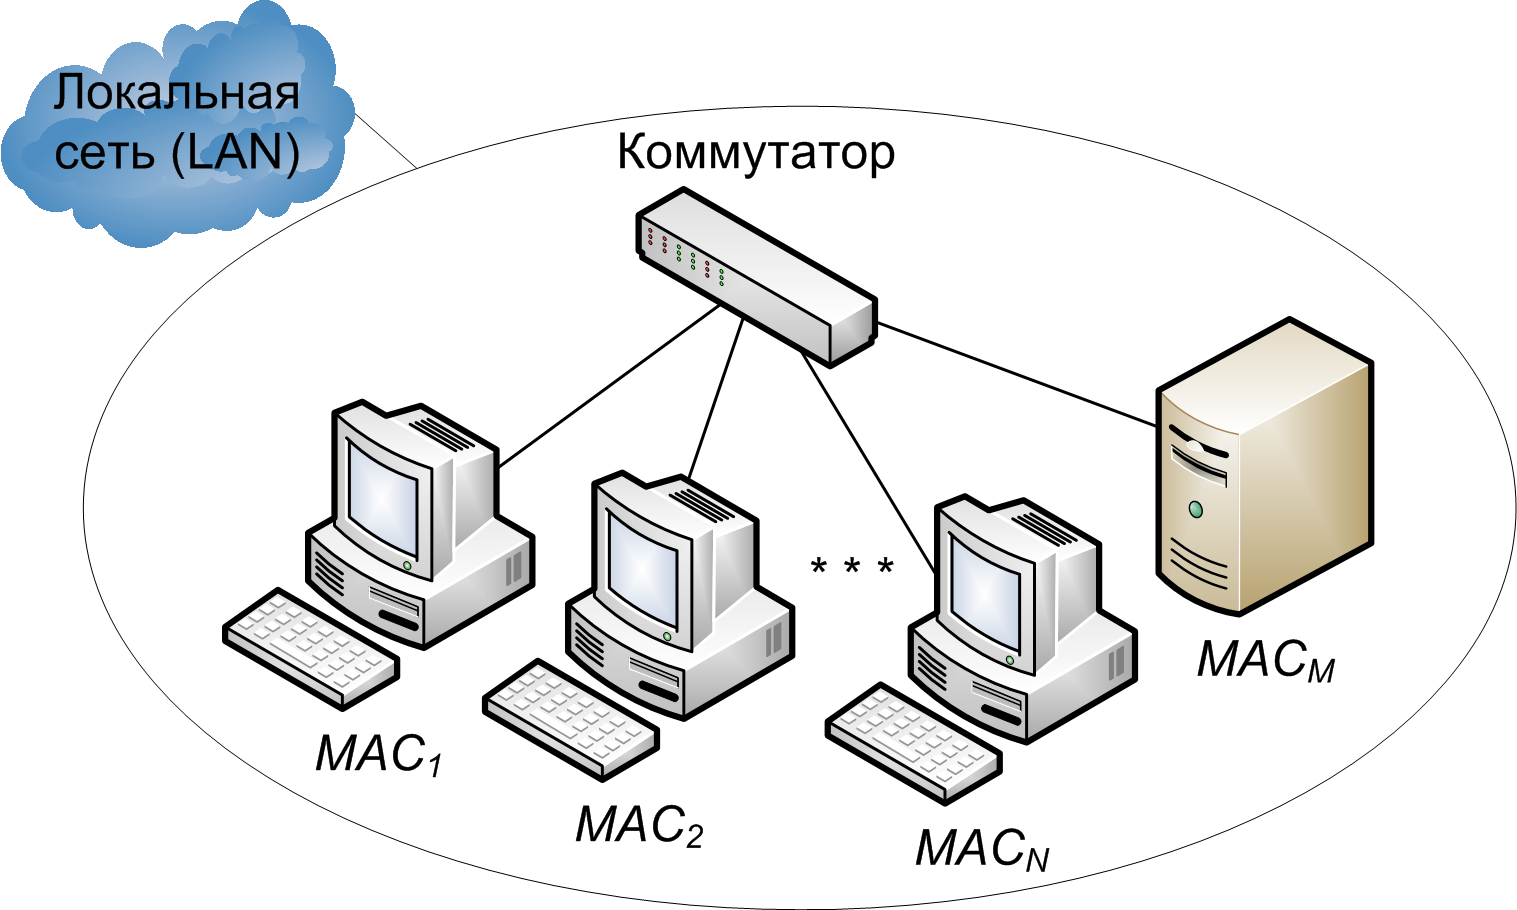
\includegraphics[width=.9\textwidth]{fig/lan}\\
    \end{figure}
\end{frame}

\begin{frame}
    \frametitle{Глобальная сеть. \alert{Internet}working}
    \framesubtitle{Адресация сетевого уровня}
    
    \begin{figure}
        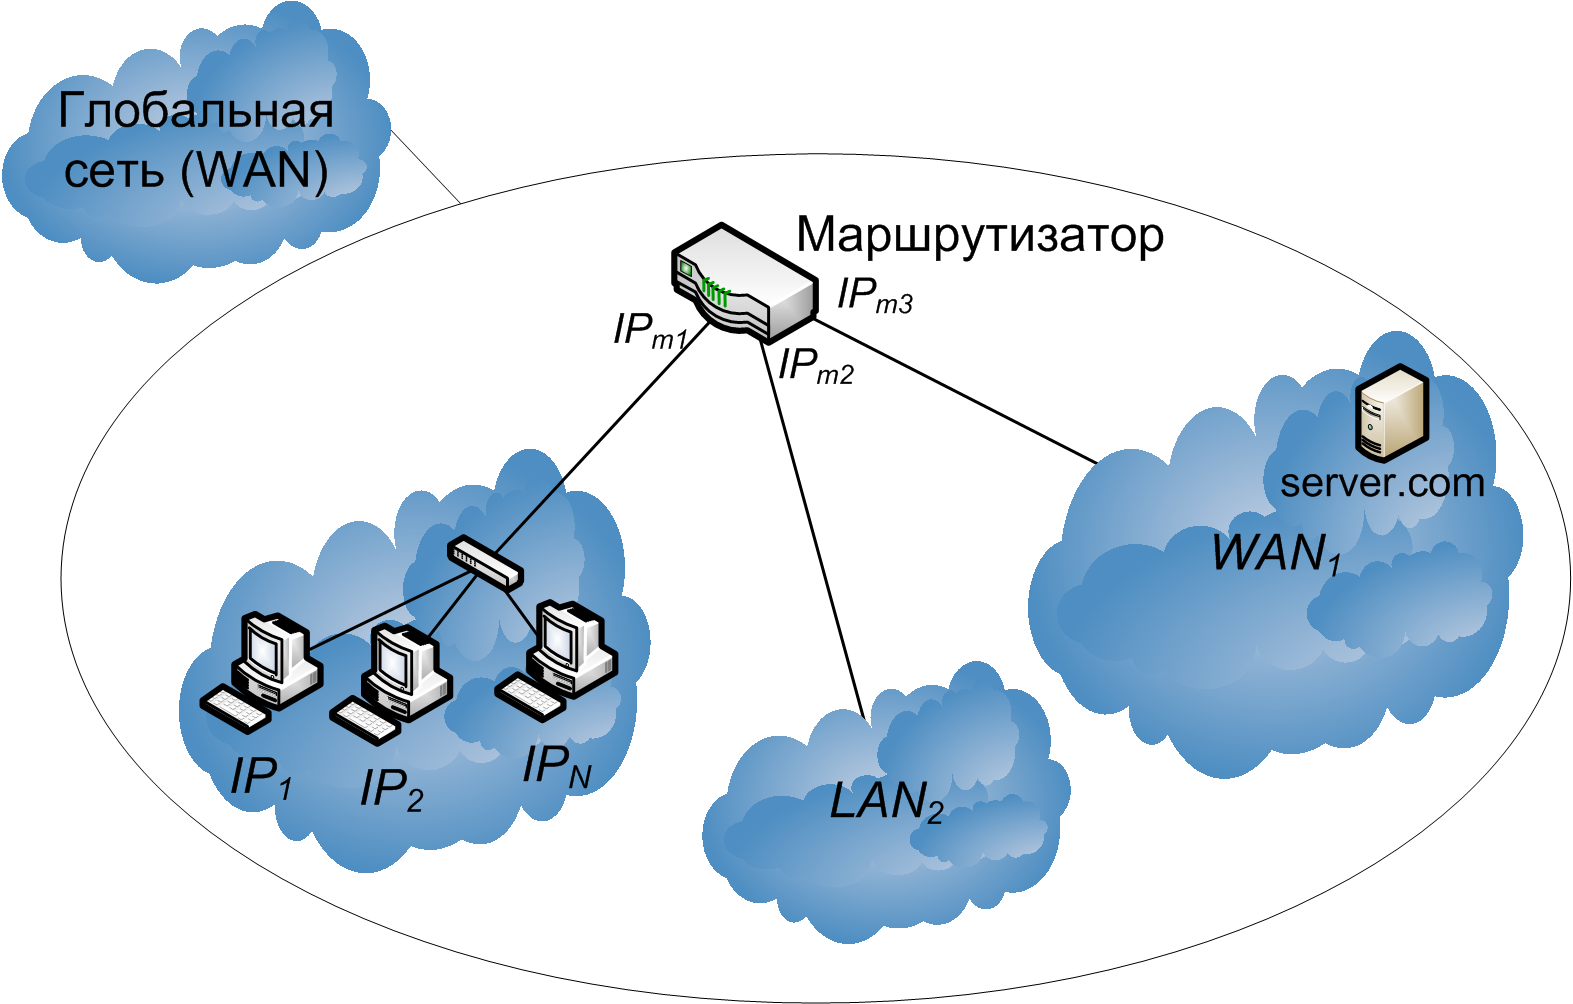
\includegraphics[width=.9\textwidth]{fig/wan}\\
    \end{figure}
\end{frame}

Отображение сетевого адреса на канальный \emph{необходимо}: иначе объединение локальных сетей чрезмерно затруднится конфликтами и изменениями.

\begin{frame}
    \frametitle{Важнейшие протоколы трансляции адресов}
    
    \begin{enumerate}
        \item ARP (Address Resolution Protocol) осуществляет отображение \alert{сетевого} адреса узла на его \alert{канальный} адрес:
        \[ARP:IP\to MAC.\]
        Например: $ARP=\{\alert{\text{192.168.100.101}}\mapsto \alert{\text{00-24-54-AA-84-AA}},\ldots\}$
        
        \item DNS (Domain Name System)\footnote{Всё шире используется Dynamic DNS (DDNS)} осуществляет отображение \alert{прикладного} адреса узла на его \alert{сетевой} адрес:
        \[DNS:DOMAIN\to IP.\]
        Например: $DNS=\{\alert{\text{mail.ru}}\mapsto \alert{\text{94.100.191.204}},\ldots\}$
    \end{enumerate}
    Подмена значений называется \alert{спуфингом} (spoofing)\footnote{Выделяют атаки ARP-spoofing и DNS-spoofing}.
\end{frame}


\section{Угрозы в сети}


\subsection{Угрозы, исходящие из сети}


\begin{frame}
    \frametitle{Угрозы, исходящие из публичной сети}
    
    \begin{itemize}
        \item Заражение вирусами.
        \item Доступ к внутренним сервисам локальной сети.
        \item Возможность реализации DOS/DDOS-атак.
        \item Сбои в работе протоколов из-за получения умышленно искажённых пакетов.
        \item Раскрытие параметров системы.
        \item Перехват и анализ сетевого трафика.
        \item Искажение передаваемых данных.
    \end{itemize}
\end{frame}


\section{Средства защиты}


\subsection{Трансляция сетевых адресов}

\begin{frame}
    \frametitle{NAT (Network Address Translation)}
    
    \begin{figure}
        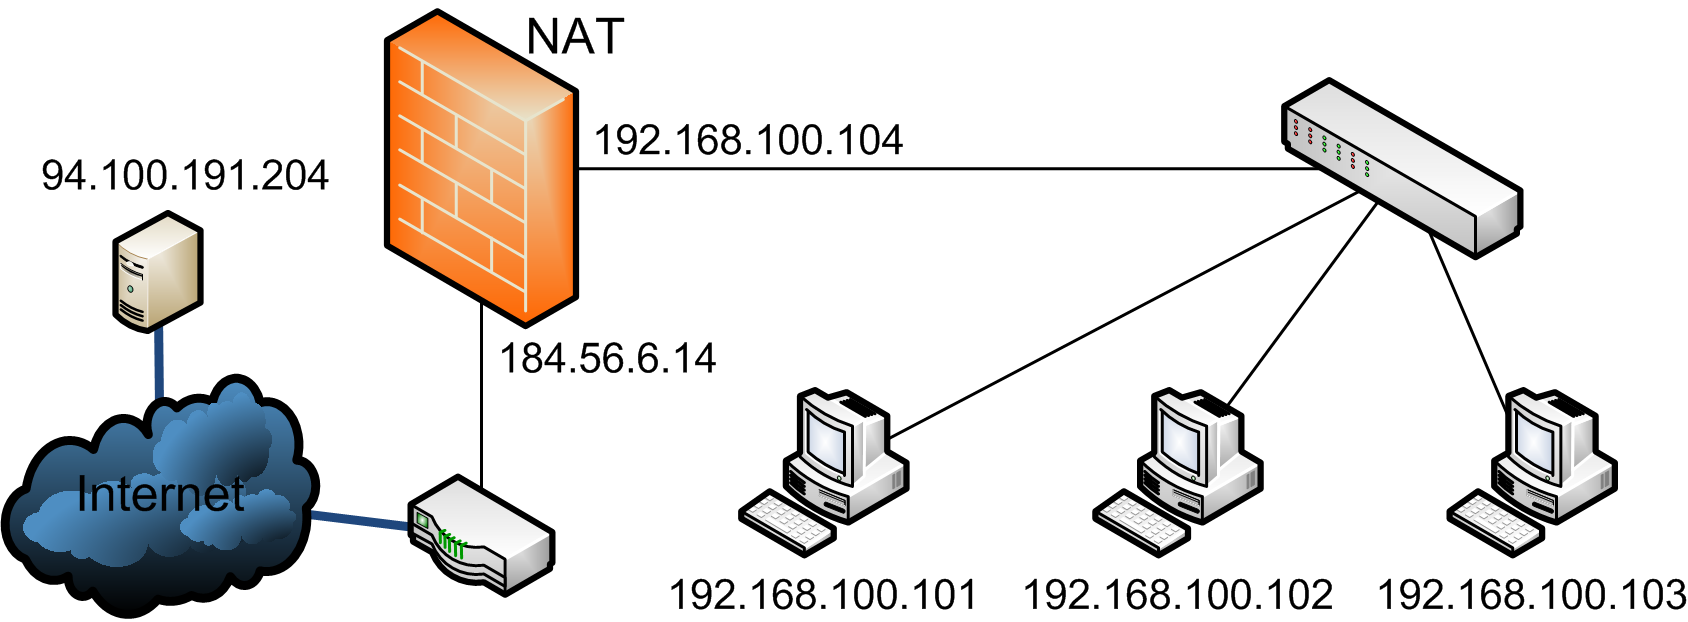
\includegraphics[width=.9\textwidth]{fig/nat}\\
    \end{figure}
    \invisible<1>{
    \begin{table}
        \centering
        \resizebox{\textwidth}{!}{
            \begin{tabular}{ccccc}
                Client && NAT && Server \\
                \only<1,2>{\visible<2>{
                    \begin{tabular}{r|l|}
                        \cline{2-2}
                        tgt & 94.100.191.204:80     \\ \cline{2-2}
                        src & 192.168.100.101:1225  \\ \cline{2-2}
                        dat & get mail.ru\ldots     \\ \cline{2-2}
                    \end{tabular}
                }}
                \only<3>{
                    \begin{tabular}{r|l|}
                        \cline{2-2}
                        tgt & 192.168.100.101:1225  \\ \cline{2-2}
                        src & 94.100.191.204:80     \\ \cline{2-2}
                        dat & <html>\ldots          \\ \cline{2-2}
                    \end{tabular}
                }
                &
                \only<1,2>{\visible<2>{$\to$}}\only<3>{$\gets$}
                &
                \visible<2,3>{
                    \begin{tabular}{r|l|}
                        \cline{2-2}
                        tgt      & 94.100.191.204:80        \\ \cline{2-2}
                        src      & 192.168.100.101:1225     \\ \cline{2-2}
                        nat      & 184.56.6.14:\alert{5000} \\ \cline{2-2}
                    \end{tabular}
                }
                &
                \only<1,2>{\visible<2>{$\to$}}\only<3>{$\gets$}
                &
                \only<1,2>{\visible<2>{
                    \begin{tabular}{r|l|}
                        \cline{2-2}
                        tgt & 94.100.191.204:80         \\ \cline{2-2}
                        src & 184.56.6.14:\alert{5000}  \\ \cline{2-2}
                        dat & get mail.ru\ldots         \\ \cline{2-2}
                    \end{tabular}
                }}
                \only<3>{
                    \begin{tabular}{r|l|}
                        \cline{2-2}
                        tgt & 184.56.6.14:\alert{5000}  \\ \cline{2-2}
                        src & 94.100.191.204:80         \\ \cline{2-2}
                        dat & <html>\ldots              \\ \cline{2-2}
                    \end{tabular}
                }
            \end{tabular}
        }
    \end{table}
    }
\end{frame}


\subsection{Межсетевое экранирование}

\begin{frame}
    \frametitle{Задачи, решаемые межсетевыми экранами}
    
    \begin{itemize}
        \item Экранирование пакетов на разных уровнях стека.
        \item Разделение сетевых подключений.
        \item Трансляция сетевых адресов.
        \item Антивирусная защита.
        \item Аутентификация.
        \item Аудит.
        \item Обнаружение вторжений (IDS), предотвращение вторжений (IPS).
        \item Биллинг, управление учетными записями.
        \item Организация виртуальных частных сетей (VPN).
        \item Балансировка нагрузки.
    \end{itemize}
\end{frame}


\begin{frame}
    \frametitle{Структура межсетевого экрана}
    
    \begin{itemize}
        \item База правил (политика безопасности).
        \item Пакетный фильтр и инспектор состояний.
        \item Модуль аутентификации и авторизации.
        \item Журнал событий.
        \item Модуль управления.
        \item Ядро (сетевой стек).
        \item Модуль мониторинга и оповещения.
        \item Прикладные посредники (proxy).
        \item Модуль поддержки VPN.
        \item Модуль создания отчетов.
    \end{itemize}
\end{frame}


\begin{frame}
    \frametitle{Подключение межсетевых экранов}
    \framesubtitle{Базовая схема}
    
    \begin{figure}
        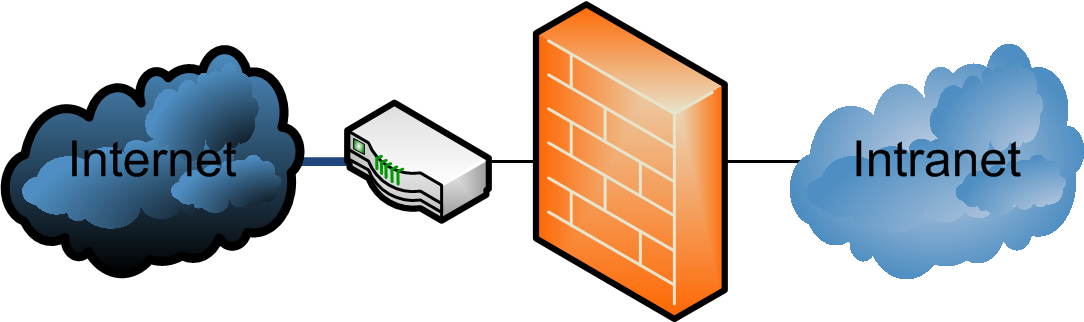
\includegraphics[width=.9\textwidth]{fig/fwallbase}\\
    \end{figure}
\end{frame}

\begin{frame}
    \frametitle{Подключение межсетевых экранов}
    \framesubtitle{Открытая подсеть}
    
    \begin{figure}
        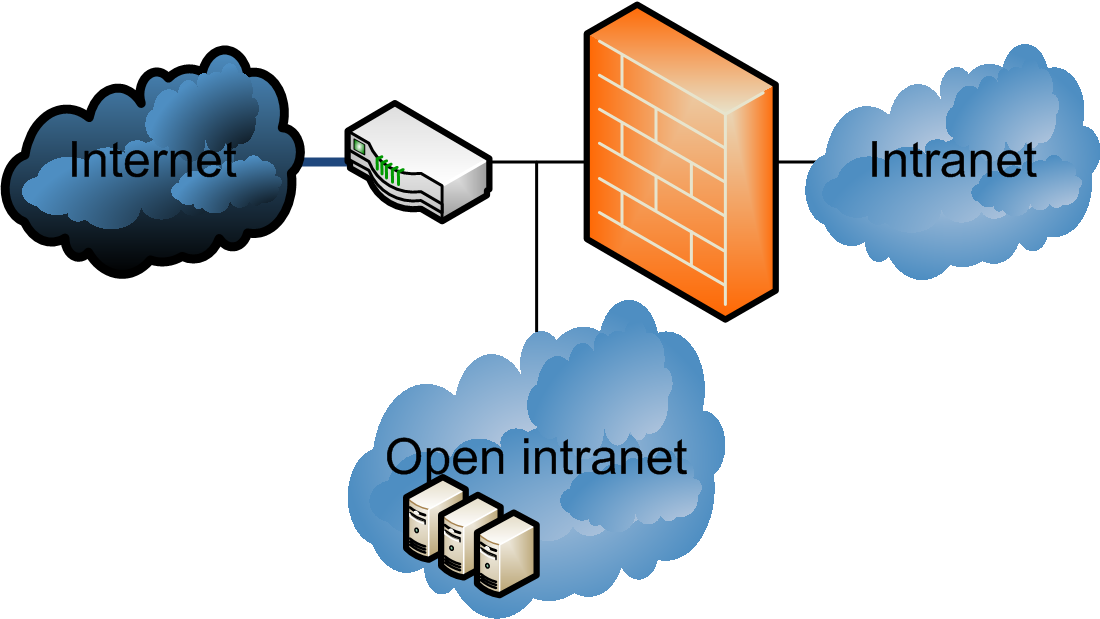
\includegraphics[width=.9\textwidth]{fig/fwallopen}\\
    \end{figure}
\end{frame}

\begin{frame}
    \frametitle{Подключение межсетевых экранов}
    \framesubtitle{Демилитаризованная зона. Экран с тремя сетевыми интерфейсами}
    
    \begin{figure}
        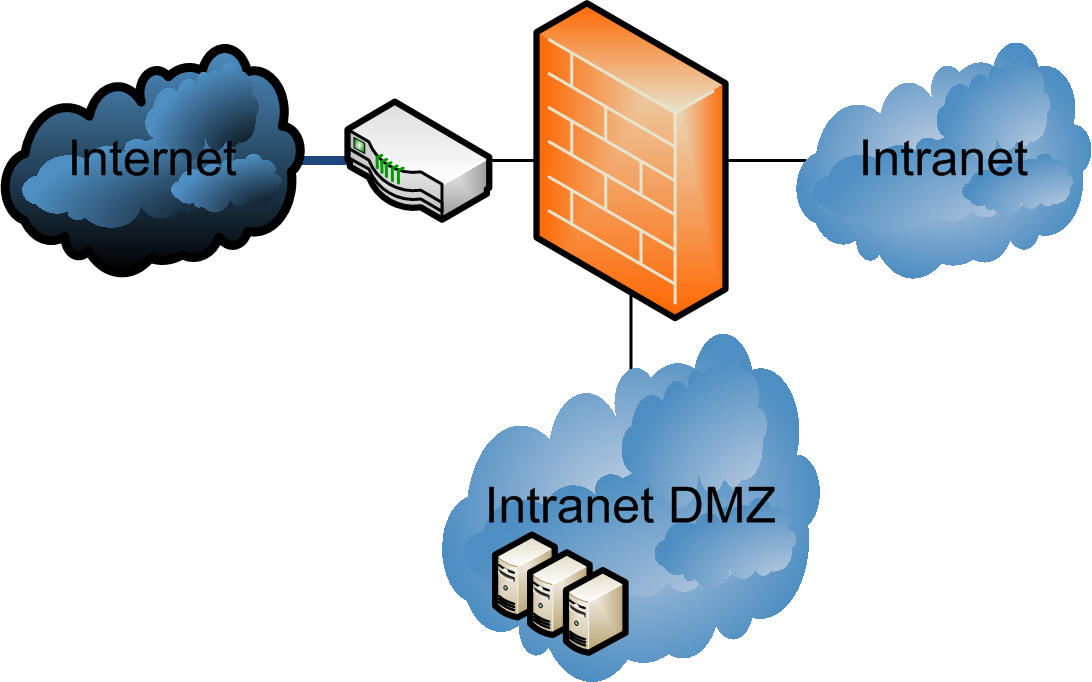
\includegraphics[width=.9\textwidth]{fig/fwalldmz}\\
    \end{figure}
\end{frame}

\begin{frame}
    \frametitle{Подключение межсетевых экранов}
    \framesubtitle{Демилитаризованная зона. Экраны с двумя сетевыми интерфейсами}
    
    \begin{figure}
        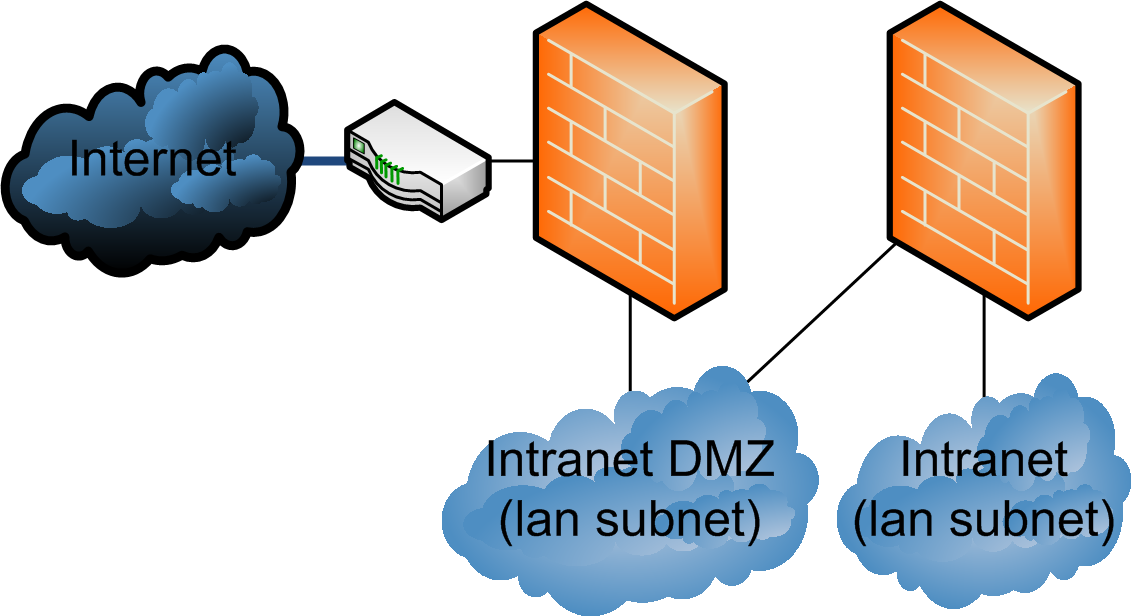
\includegraphics[width=.9\textwidth]{fig/fwalldmzlan}\\
    \end{figure}
\end{frame}


\subsection{Аутентификация и VPN}

\begin{frame}
    \frametitle{VPN}
    \framesubtitle{Организация защищенного канала связи через публичную сеть}
    
    \begin{figure}
        \only<1>{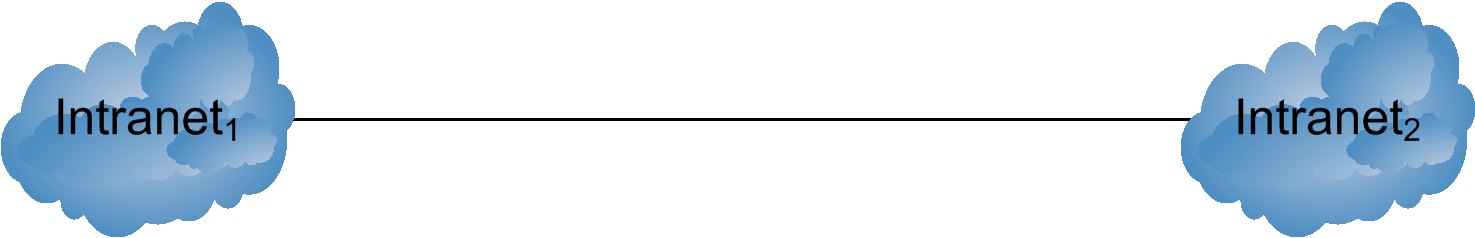
\includegraphics[width=.9\textwidth]{fig/intranet}}
        \only<2>{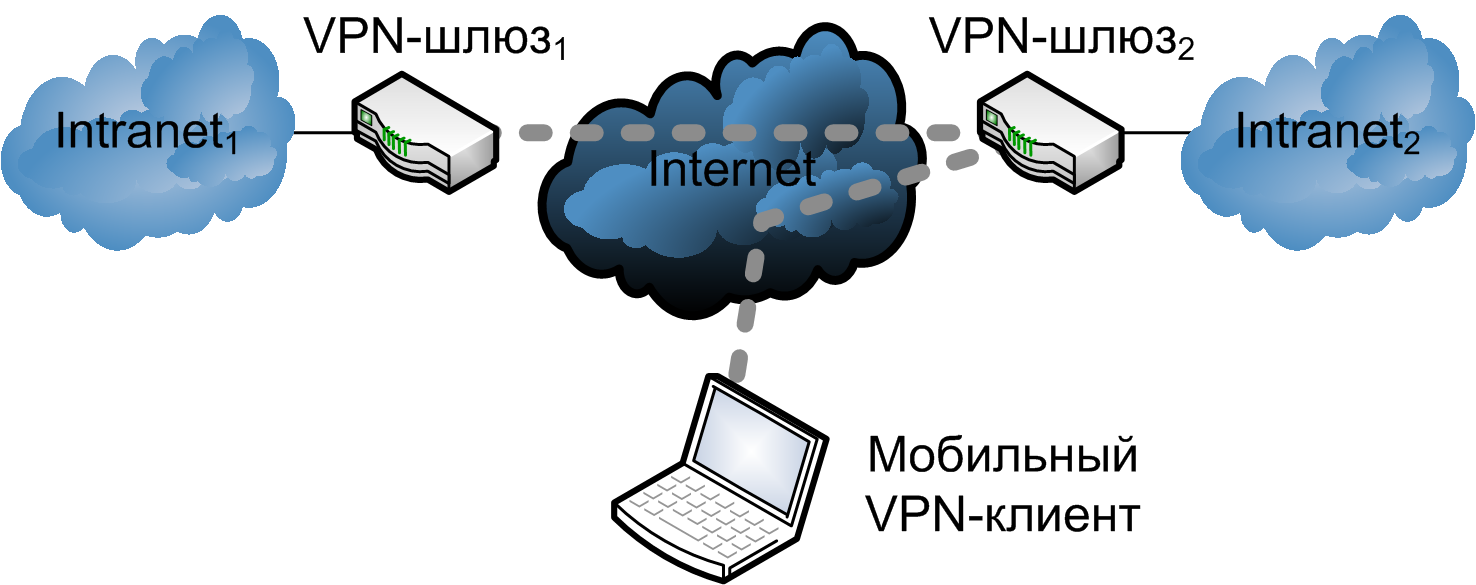
\includegraphics[width=.9\textwidth]{fig/vpn}}
    \end{figure}
\end{frame}

\begin{frame}
    \frametitle{Протоколы для организации защищенных соединений}

    \begin{table}
        \centering
        \begin{tabular}{|l|l|}
            \hline\hline
            Уровень TCP/IP              & Протокол  \\
            \hline\hline
            Прикладной                  &           \\ \hline            
            Представительный            & SSL/TLS   \\ \hline            
            Сеансовый                   & SOCKS     \\ \hline            
            Транспортный                &           \\ \hline            
            Сетевой                     & IPSec     \\ \hline
            Канальный                   & PPTP, L2TP\\ \hline            
            Физический                  &           \\ \hline
        \end{tabular}
    \end{table}    
\end{frame}


\begin{frame}
    \frametitle{VPN:Туннелирование ip-трафика (IPSec)}
    
    \begin{figure}
        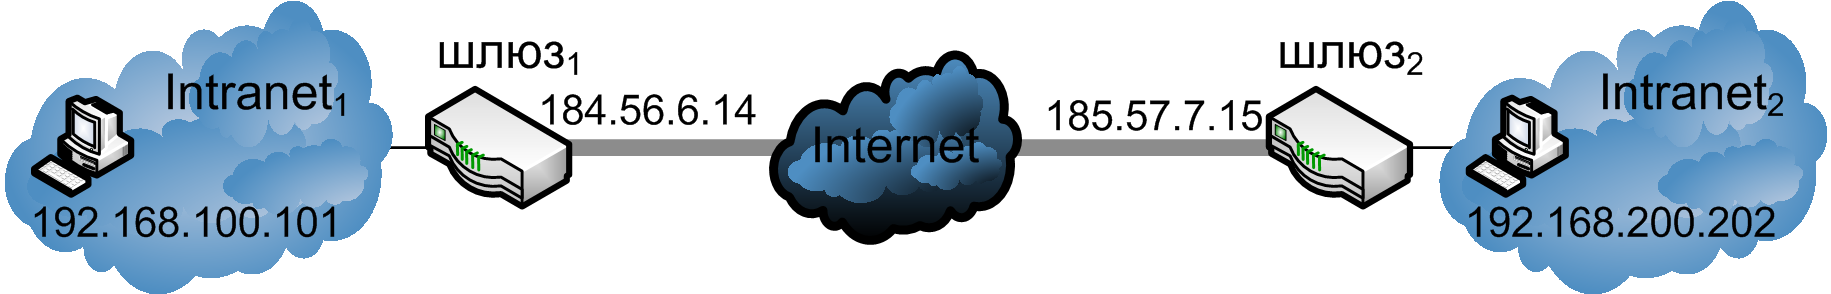
\includegraphics[width=.9\textwidth]{fig/vpntunnel}
    \end{figure}
    \begin{table}
        \centering
        \resizebox{.9\textwidth}{!}{
            \begin{tabular}{lcccc}
                \hline\hline
                Стек      &192.168.100.101&$\text{Шлюз}_1$&$\text{Шлюз}_2$&192.168.200.202\\
                \hline\hline
                5.Пр
                    &\uncover<1,13>{$M$}
                        &&
                                &\uncover<12,13>{$M$}
                                    \\
                4.Тр
                    &\uncover<2,13>{$h_4Mt_4$}
                        &&
                                &\uncover<11,13>{$h_4Mt_4$}
                                    \\
                3.Сет
                    &\only<3,13>{$h_3h_4Mt_4h_3$}\only<4>{$M_{IP}$}
                        &\only<5>{$M_{IP}$}\only<6>{$h'_3\{M_{IP}\}_kt'_3$}
                            &\only<7>{$h'_3\{M_{IP}\}_kt'_3$}\only<8>{$M_{IP}$}\only<9>{$h_3h_4Mt_4h_3$}
                                &\uncover<10,13>{$h_3h_4Mt_4h_3$}
                                    \\
                2.Кан
                    &\uncover<5,13>{$\downarrow$}
                        &\only<5>{$\uparrow$}\only<7>{$\downarrow$}
                            &\only<7>{$\uparrow$}\only<10>{$\downarrow$}
                                &\uncover<10,13>{$\uparrow$}
                                    \\
                1.Физ
                    &\uncover<5,13>{$\downarrow$}
                        &\only<5>{$\uparrow$}\only<7>{$\downarrow$}
                            &\only<7>{$\uparrow$}\only<10>{$\downarrow$}
                                &\uncover<10,13>{$\uparrow$}
                                    \\
                \hline
                    &\uncover<3,4,5,13>{t:192.168.200.202}
                        &\uncover<6,7>{t:185.57.7.15}
                            &\uncover<8,9,10>{t:192.168.200.202}
                                &\invisible{t:192.168.200.202}
                                    \\
                    &\uncover<3,4,5,13>{s:192.168.100.101}
                        &\uncover<6,7>{s:184.56.6.14}
                            &\uncover<8,9,10>{s:192.168.100.101}
                                &\invisible{s:192.168.100.101}
            \end{tabular}
        }
    \end{table}
\end{frame}

%TODO ipsec, ssl/tls

\appendix


\section{Источники}

\begin{frame}
    \frametitle{Источники}
    
    Рекомендуется к прочтению базовые книги по сетям \cite{bib:olifers:networks,bib:tannen:networks}. О сетевой безопасности см \cite{bib:shangin:2012:secInNetworks}. Хорошим введением в защиту периметра будет несколько устаревшая \cite{bib:lebed:2002:firewalls}.
\end{frame}

\section{Библиография}

\begin{frame}[allowframebreaks]{Библиография}
    \bibliographystyle{gost780u}
    \bibliography{./../bibliobase}
\end{frame}


\end{document}